\documentclass{article}
 
\usepackage[T2A]{fontenc}
\usepackage[utf8]{inputenc}
\usepackage[bulgarian]{babel}
\usepackage{cite}
\usepackage{graphicx}
\usepackage{amsmath}
\usepackage{amsfonts}
\usepackage{float}
\usepackage{pgfplots}
\usepackage{amssymb}

\graphicspath{{images/}}

\title{Изследване на скалируемостта на Wa-Tor симулацията при cтатична декомпозиция на домейна}

\author{Иван-Асен Веселинов Чакъров \\
	ФН: 81837, Курс: 3, Група: 1}
\date{Юли 2021}


\begin{document}

\maketitle

\section{Увод}
Wa-Tor~\cite{wator} е класически проблем при паралелното програмиране.
Накратко проблемът е симулирането на идеализиран двумерен свят с формата на тор.
Светът има два вида обитатели - херинги, които играят ролята на плячка и акули, които ловят и изяждат херингите.
Подробните правилата за симулацията са дадени във~\cite{wator}.
\\
\\
Декомпозицията на домейн (Domain decomposition)~\cite{domain_decomposition}
при паралелното програмиране се явява естествен подход при решаването на проблеми,
при които за решаването на проблема за даден елемент $D$ от домейна са нужни само малко подмножество от данни,
които са "близо" до $D$. Накратко, идеята е, че разбиваме домейна на множество поддомейни
и възлагаме решаването на проблема за всеки поддомейн на отделен процес.
Важно е отделните поддомейни да са със еднаква големина за да може да се разпредели
хубаво работата между процесорите. Съществуват два вида Domain decomposition - статичен и динамичен.
При статичния в началото на алгоритъма разбиваме домейна и разпределяме работата между процесите.
По време на симулацията разбиването не се променя, което може да води до намаляване на производителността
тъй като данните при доста проблеми прескачат от един домейн в друг.
Този проблем се решава от втория тип Domain decomposition, който по време на симулацията
преизчислява разбиването на домейна с цел балансиране на големината на отделните поддомейни.
Domain decomposition намира приложение при решаването на проблеми от тип
Celular automata ~\cite{celular_automata}.
\\
\\
Тъй като и Wa-Tor попада в този тип проблеми, решението което представям тук е базирано
на статична декомпозиция на домейна.
\\
\\
разбивеме светът по редове (или по колони) на равни по големин ленти.

\section{Архитектура}
Решението е имплементирано на Java 16 и използва вградени способности за паралелно програмиране,
част от Java SE.
\begin{itemize}
	\item java.lang.Thread: основният начин за създаване на нишки във Java
	\item java.util.concurrent.ExecutorService
	\item java.util.concurrent.locks.ReentrantLock
\end{itemize}

Архитектурата използва статична декомпозиция на домейна и е по модела Master-Slaves.

\begin{figure}[H]
	\centering
	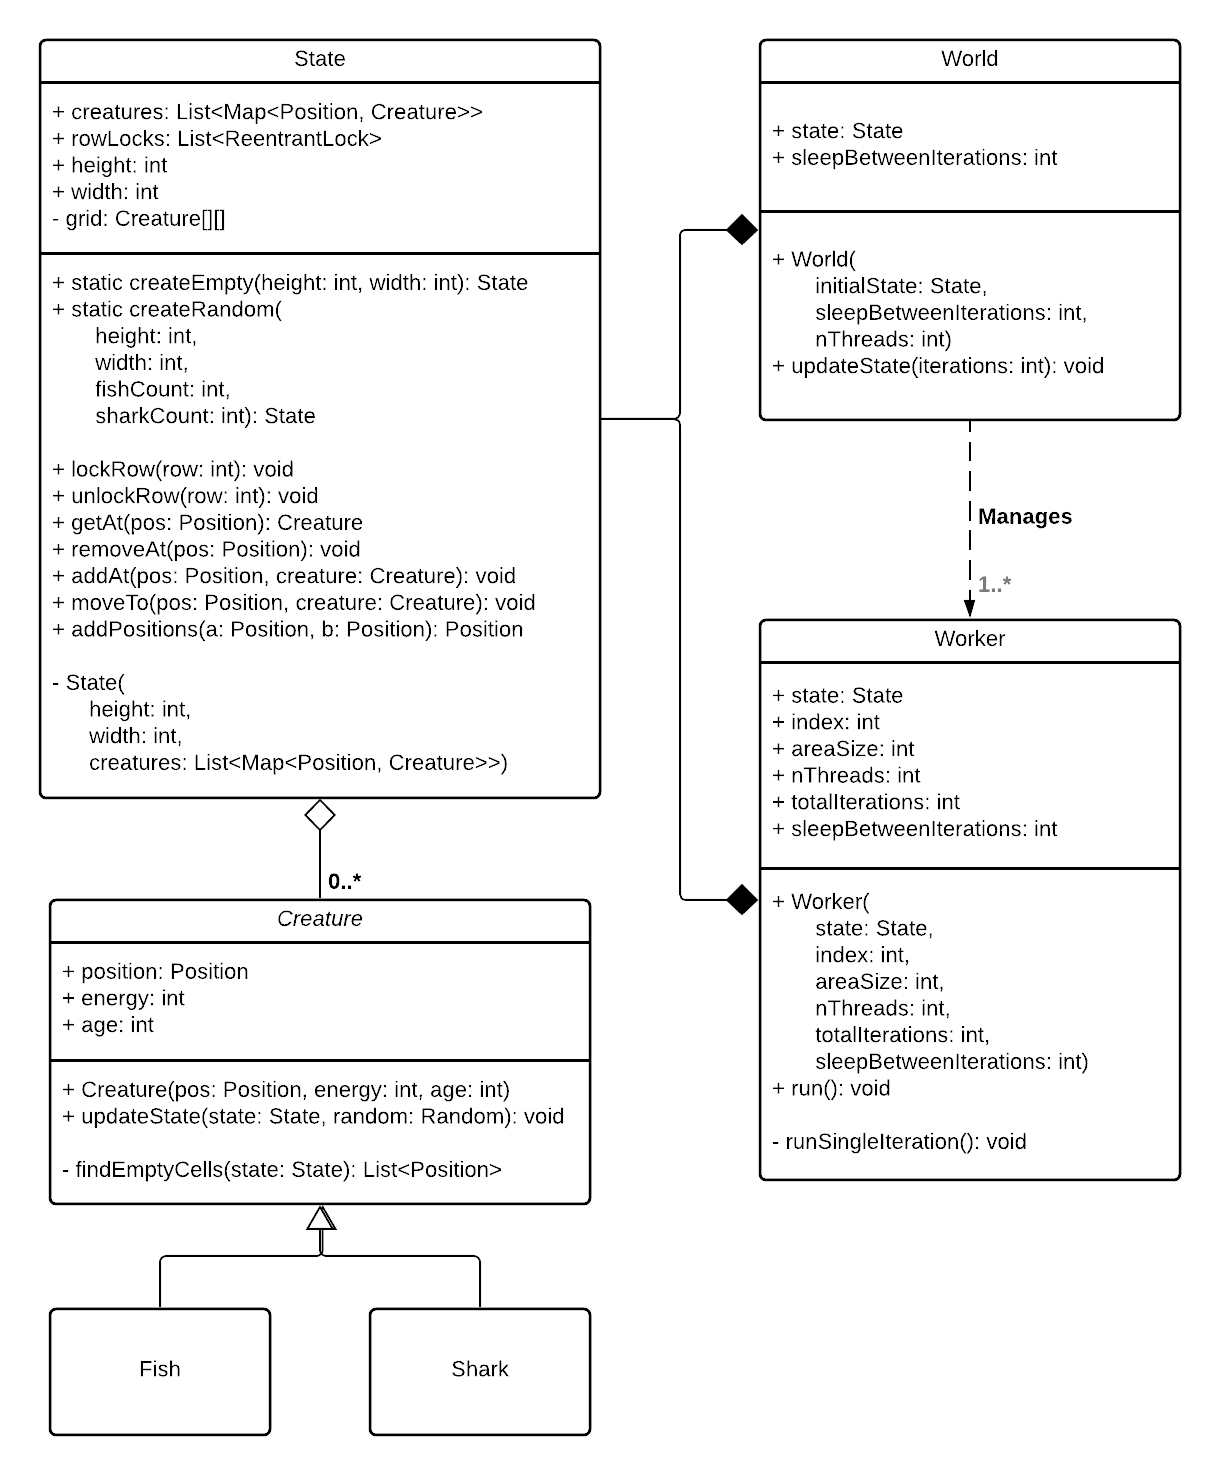
\includegraphics[width=1.1\textwidth]{classes-uml.png}
	\caption{UML Клас диаграма на проекта}
	\label{fig:figure1}
\end{figure}

\section{Тестови резултати}

Характеристики на тестовата машина: 

\begin{tabular}{ |p{3cm}||p{3cm}|p{3cm}|p{3cm}|  }
 \hline
 \multicolumn{4}{|c|}{Ускорение (MIN,AVG,MAX) при размер 4000x2000 и популация 1 000 000} \\
 \hline
 Брой нишки & MIN & AVG & MAX \\
 \hline
 1  & 1.00  & 1.00  & 1.00 \\
 6  & 4.78  & 4.89  & 4.93 \\
 11 & 7.08  & 7.38  & 7.50 \\
 16 & 8.44  & 8.63  & 8.65 \\
 21 & 9.24  & 9.41  & 9.36 \\
 26 & 9.61  & 10.00 & 10.04 \\
 31 & 10.12 & 10.32 & 10.39 \\
 \hline
\end{tabular}

\begin{tikzpicture}
\begin{axis}[
	title={Време за изпълнение при размер на полето 4000x2000},
	xlabel={Брой нишки},
	ylabel={Време в секунди},
	legend pos=north west,
	ymajorgrids=true,
	grid style=dashed,
]

\addplot[
	color=blue,
	mark=square,
	]
	coordinates {
	(1,517)(6,105)(11,70)(16,59)(21,54)(26,51)(31,50)
	};

\end{axis}
\end{tikzpicture}

\begin{tikzpicture}
\begin{axis}[
	title={Средно ускорение при размер на полето 4000x2000},
	xlabel={Брой нишки},
	ylabel={Ускорение},
	legend pos=north west,
	ymajorgrids=true,
	grid style=dashed,
]

\addplot[
	color=blue,
	mark=square,
	]
	coordinates {
	(1,1)(6,4.9)(11,7.4)(16,8.6)(21,9.4)(26,10)(31,10.3)
	};
\addlegendentry{Реално ускорение}

\addplot[
	domain=0:31,
	color=green
]{0.7 * x};
\addlegendentry{Идеално ускорение}
\end{axis}
\end{tikzpicture}

\section{Визуализации}
Освен симулацията, която служи за измервание на скалируемостта,
в проекта е разработена и визуализация в реално време с помощта на Java Swing и AWT.
Следват няколко екранни снимки от визуализации (херингите са в зелено, а акулите в синьо):

\begin{figure}[H]
	\centering
	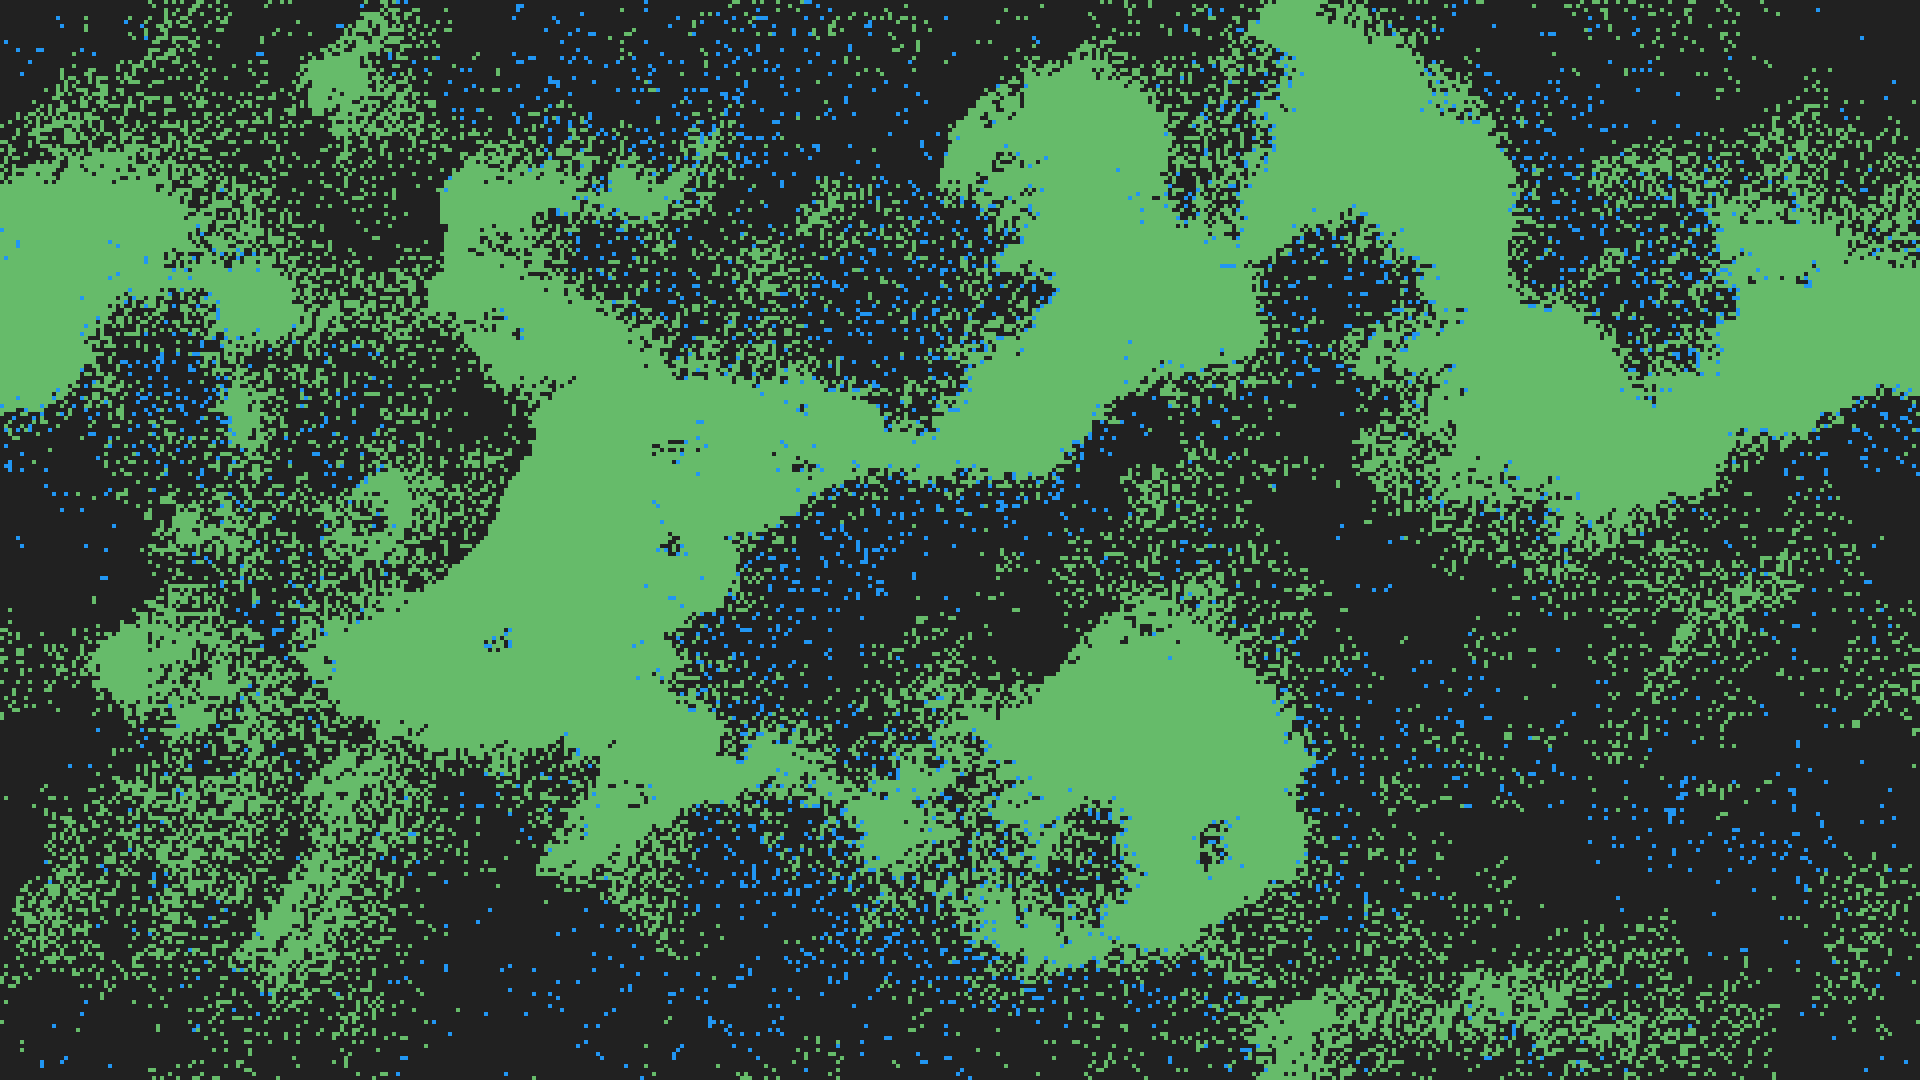
\includegraphics[width=1\textwidth]{screenshot-small.png}
	\caption{Размер на полето 480x270, 10 000 херинги и 1000 хиляди акули}
\end{figure}

\begin{figure}[H]
	\centering
	
\includegraphics[width=1\textwidth]{screenshot-big.png}
	\caption{Размер на полето 1920x1080, 1 000 000 херинги и 100 000 акули}
\end{figure}

Първоначалната цел на този "режим на работа" беше лесен начин за дебъгване,
но в крайна сметка се получи и доста готина анимация, която би могла да се ползва за screensaver :).

\section{Бъдещо развитие на проекта}
Използване на Dynamic domain decomposition

\bibliography{wator}{}
\bibliographystyle{plain}
\end{document}
